

\section{The Proposed \Ours}

\subsection{Problem Definition}


% Let $\mathbb{D} = \{(X^1,y^1),(X^2,y^2),...,(X^n,y^n)\}$ denote a dataset comprising $n$ temporal observation pairs, where each $X^i \in \mathbb{R}^{t \times m}$ represents a multivariate time series with $t$ time steps and $m$ features, and $y^i \in \mathbb{R}^{h \times d}$ corresponds to the $d$-dimensional target values over $h$ future time steps. The objective of time series forecasting task is to learn a predictive model $f_\theta: \mathbb{R}^{t \times m} \rightarrow \mathbb{R}^{h \times d}$ that captures the temporal dependencies in $\mathbb{D}$.
% Within \Ours framework, we propose a prompt specifically designed for time series forecasting tasks. Let $P$ be a task-specific prompt template, the model's forecasting procedure can be formalized as:
% $ T^i = \text{LLM}_\phi(P, X^i) $
% where $T^i$ denotes the textual output generated by LLMs with parameters $\phi$ given the prompt $P$ and input time series $X^i$. The predicted future values $\hat{y}^i \in \mathbb{R}^{h \times d}$ are subsequently obtained through a deterministic parsing function $g$ that transforms the textual output $T^i$ into numerical predictions:
% $ \hat{y}^i = g(T^i) $.

% Let $\mathbb{D} = \{(X^i,y^i)\}_{i=1}^n$ be a temporal dataset, where each $X^i \in \mathbb{R}^{t \times m}$ is a multivariate time series with $t$ steps and $m$ channels, and $y^i \in \mathbb{R}^{h \times d}$ contains $d$-dimensional targets over $h$ future steps. The forecasting task learns a mapping $f_\theta: \mathbb{R}^{t \times m} \rightarrow \mathbb{R}^{h \times d}$ capturing temporal dependencies in $\mathbb{D}$. Under \Ours, the forecasting procedure using prompt template $P$ is: $T^i = \text{LLM}_\phi(P, X^i)$, where $T^i$ is the LLM's textual output, and $\hat{y}^i = g(T^i)$ parses it into numerical predictions $\hat{y}^i \in \mathbb{R}^{h \times d}$.

Let $\mathbb{D} = \{(X^i,y^i)\}_{i=1}^n$ be a temporal dataset, where each $X^i \in \mathbb{R}^{t \times m}$ is a multivariate time series with $t$ steps and $m$ channels, and $y^i \in \mathbb{R}^{h \times d}$ contains $d$-dimensional targets over $h$ future steps. The forecasting task learns a mapping $f_\theta: \mathbb{R}^{t \times m} \rightarrow \mathbb{R}^{h \times d}$ capturing temporal dependencies in $\mathbb{D}$. Under \Ours, the forecasting procedure using prompt template $P$ is: $T^i = \text{LLM}_\phi(P, X^i)$, where $T^i$ is the LLM's textual output, and $\hat{y}^i = g(T^i)$ parses it into numerical predictions $\hat{y}^i \in \mathbb{R}^{h \times d}$. Here, $g: \mathcal{T}\rightarrow \mathbb{R}^{h \times d}$ denotes a deterministic parsing function that extracts $h\!\cdot\! d$ real-valued numbers from $T^i$ and reshapes them into an $h \times d$ matrix.


\subsection{\Ours Overview}

\Ours consists of a two-stage RFT framework for LLM-based time series forecasting, built upon a structured training template that standardizes input representations and encodes task-specific knowledge. In the first stage, we perform warm-up SFT using synthetic chain-of-thought trajectories to teach the model effective temporal analysis and accurate output formatting. These trajectories are generated under strict guidelines and refined iteratively to align with ground-truth forecasts. The second stage further improves the model via RL, guided by a fine-grained, multi-objective reward function tailored for time series forecasting. To optimize reasoning paths during RL, we introduce GRIP (Group-based Relative Importance for Policy Optimization), a novel strategy that leverages non-uniform sampling and adaptive weighting to balance accuracy, logical consistency, and temporal coherence. An overview of the framework is provided in Figure \ref{fig:1_framework}.

% \begin{table*}[h]\centering
% \vspace{-0.1in}
%     \caption{TODO}
%     \label{tab:main_results}
%     \renewcommand{\arraystretch}{1}
%     \resizebox{0.98\textwidth}{!}{
%     \large
%     \begin{tabular}{l}
%         \toprule
%          Here is the <Channel Information> data of the ETTh1 dataset. The ETTh1 dataset is a <Dataset Information>.  I will now give you data for the past 96 recorded dates, and please help me forecast the data for the next 96 recorded dates. The data is as follows: <Historical Time Series Data> Please give me the complete data for the next 96 recorded dates. Remember to give me the complete data. You must first conduct reasoning inside <think> ...</think>. When you have the final answer, you can output the answer inside <answer>...</answer>.  \\
%         \bottomrule
%     \end{tabular}
% }
% \vspace{-0.15in}
% \end{table*}


\begin{table}[ht]
\centering

\caption{Training prompt template for Time-R1. Contents enclosed in \{\} will be replaced with specific information, including dataset description, channel information, and historical time-series data.} 
\vspace{-0.08in}
\label{tab:training_template}
\renewcommand{\arraystretch}{0.9}
\begin{tabular}{@{} p{0.5\dimexpr\textwidth-4\tabcolsep} @{}}
\toprule
Here is the \blue{\{Channel Information\}} data of the ETTh1 dataset. The ETTh1 dataset is \lightblue{\{Dataset Description\}}. I will now give you data for the past 96 recorded dates, and please help me forecast the data for the next 96 recorded dates accurately. The data is as follows: \khaki{\{Historical Time Series Data\}}. Please give me the complete data for the next 96 recorded dates in chronological order. Remember to give me the complete data without omission. You must first conduct reasoning inside \pink{<think>}...\pink{</think>}. When you have the final answer, you can output the answer inside \red{<answer>}...\red{</answer>}. \\
\bottomrule
\end{tabular}
\vspace{-0.08in}
\end{table}


\vspace{-0.12in}
\subsection{Training Template}


Our training template standardizes inputs and encodes task-specific knowledge through five carefully designed components: (1) \textit{Task Definition} establishing objectives and problem scope; (2) \textit{Dataset Description} specifying temporal characteristics and application scenarios; (3) \textit{Channel Information} which delineates the types and semantic meanings of input signals; (4) \textit{Testing Data} providing timestamps and historical series; and (5) \textit{Format Instruction} defining output templates. 
By organizing these elements into a unified prompt structure, the template interleaves domain knowledge with explicit structural constraints, enabling the model to better understand the forecasting context while reducing inference-time formatting ambiguities and response inconsistencies (see Table \ref{tab:training_template}).
% This design interleaves domain knowledge with structural constraints, reducing inference-time formatting ambiguities (see Table \ref{tab:training_template}).




\subsection{SFT for Warmup Adaptation} 
\label{SFTdata}

To mitigate the linguistic readability degradation and slow convergence caused by direct reinforcement learning on LLMs, we first perform a warmup stage via SFT. This warmup SFT step is designed to stabilize training, ensure proper output formatting, and equip the model with basic reasoning capabilities.

Our SFT data construction involves three key steps. First, we leverage DeepSeek-R1 to generate time-series predictions on the training set by feeding it historical time series data paired with strict formatting guidelines. We then select the optimal prediction for each sample based on the MSE metric. Next, to derive a reasoning process aligned with ground-truth labels, we inject both the true prediction value and the high-quality CoT generated in the previous step into DeepSeek-R1 as prompts, guiding it to synthesize a revised CoT that logically culminates in the correct prediction. Finally, we concatenate the refined CoT and the true prediction value, demarcating the final answer using `<answer>` tags to create structured training data for SFT. 
% The full data collection procedure is detailed in Algorithm \ref{alg:cot_construction} in the Appendix for completeness.

After constructing the training data, we perform a single-epoch fine-tuning. This warm-up SFT phase effectively prepares the model for  reinforcement learning, ensuring stable learning dynamics and accurate output formatting. It also enables the model to internalize reasoning patterns from synthetic trajectories, laying the foundation for more deliberate and coherent decision-making in later reinforcement learning stages.




\subsection{RL for Effective Reasoning}

% After warmup SFT, we further fine-tune the LLM using RL to generalize its reasoning and acquire slow-thinking capabilities for time series forecasting. In the following sections, we first present the reward design, and then describe the employed reinforcement learning algorithm GRIP. 

After warmup SFT, we further fine-tune the LLM with RL to improve reasoning generalization and enable slow-thinking for time series forecasting. We next introduce the reward design and the RL algorithm GRIP.


\subsubsection{Reward Design}
\label{sec:Reward Modeling}
To effectively apply RL for optimizing the proposed slow-thinking time series forecasting, we introduce several fine-grained and multi-objective reward functions specifically designed to enhance forecasting performance and slow thinking behavior. We define the total reward as a weighted sum of the following components.


\paragraph{Format Rewards.}  
To ensure syntactic validity and completeness of the generated reasoning paths, we define two reward components to enforce both structural integrity and output completeness:

\textit{Format Reward:} A binary penalty is imposed if the output does not follow the required structured format (e.g., missing or malformed \texttt{<answer>} tags):
{
\setlength{\abovedisplayskip}{5pt}
\setlength{\belowdisplayskip}{5pt}
\begin{equation}
\small
\gamma_{\text{Format}} = 
\begin{cases}
0 & \text{if valid } \texttt{<think>}, \texttt{<answer>} \text{ tags} \\
-1 & \text{otherwise}
\end{cases}
\end{equation}
}

\textit{Length Reward:} To encourage full time point sequence generation and accelerate convergence, we provide positive feedback based on how close the generated sequence length is to the ground truth:
% \begin{equation}
% \gamma_{\text{Length}} = 
% \begin{cases}
% 0.1 & \text{if } \text{len(answer)} \geq \text{len(ground\_truth)} \\
% 0.1 \cdot \dfrac{\text{len(answer)}}{\text{len(ground\_truth)}} & \text{otherwise}
% \end{cases}
% \end{equation}
{\setlength{\abovedisplayskip}{5pt}
\setlength{\belowdisplayskip}{5pt}
\begin{equation}
\gamma_{Length} = 0.1 \cdot \min \left( 1, \frac{L_a}{L_g} \right),
\end{equation}
}
where $L_a$ and $L_g$ denote the predicted-sequence length and the ground-truth-sequence length.

\begin{figure*}[t] % 浮动环境
    \centering
    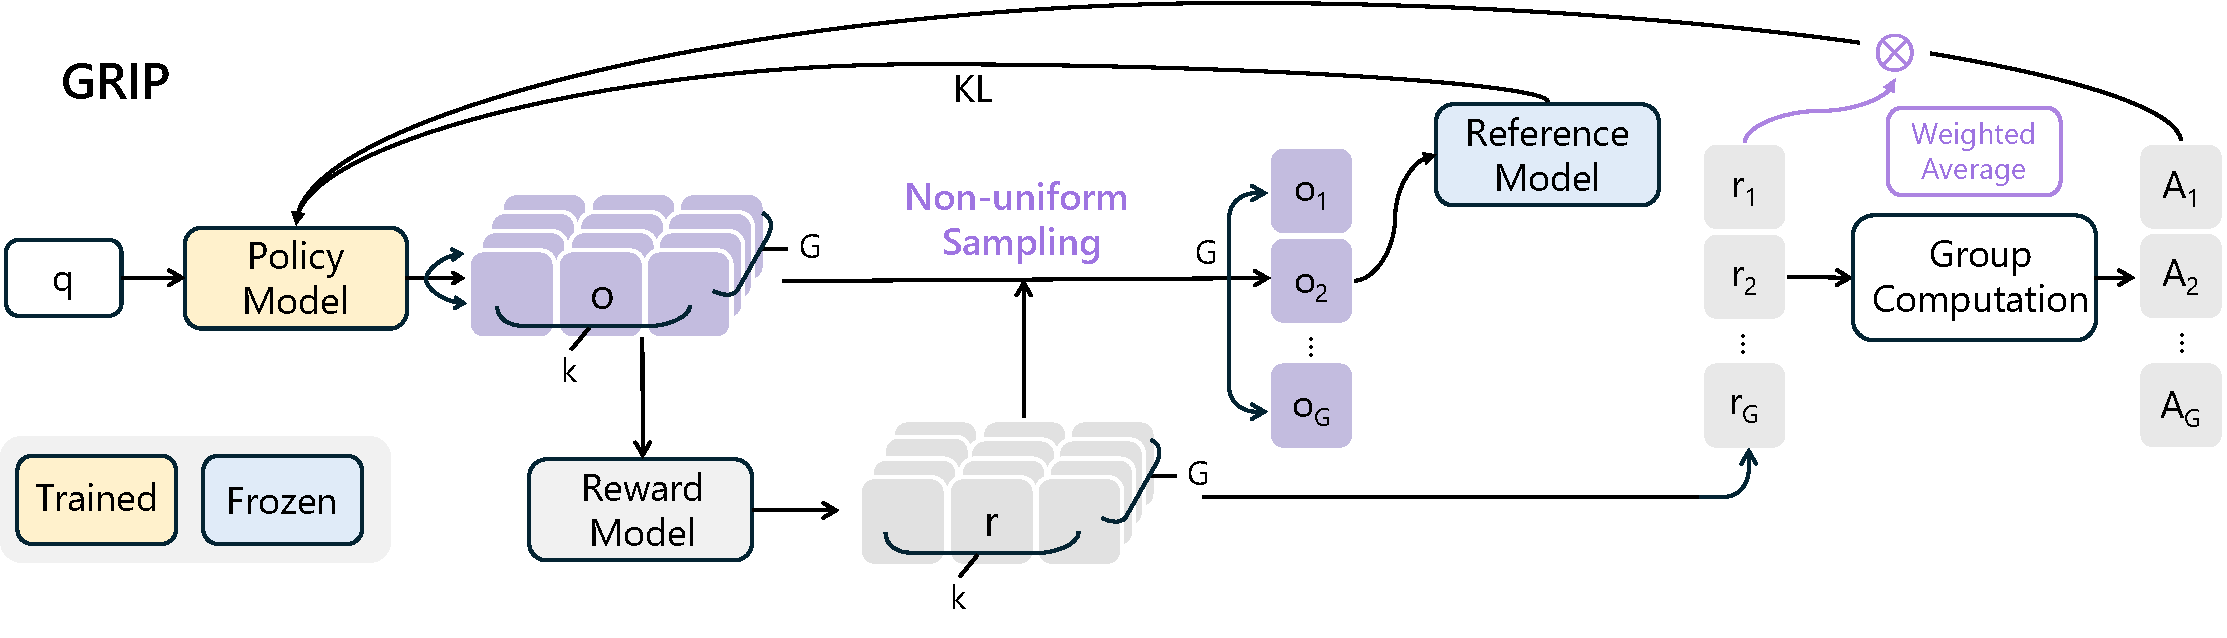
\includegraphics[width=1\textwidth, keepaspectratio]{images/2_grip_.pdf} % 调整宽度    

    \caption{Overview of Group-based Relative Importance for Policy Optimization (GRIP). } % 添加标题
    \label{fig:2_grip} % 添加标签用于引用

\end{figure*}

\paragraph{Accuracy Rewards.}
We define two accuracy-based reward components to assess numerical precision, encouraging accurate value prediction and modeling of dynamics:

\textit{MSE Reward:} We compute the mean squared error between normalized prediction and target sequences and map it into a bounded reward signal using a sigmoid transformation:
{\setlength{\abovedisplayskip}{5pt}
\setlength{\belowdisplayskip}{5pt}
\begin{equation}
\gamma_{\text{MSE}} = \left(1 - \frac{1}{1 + e^{-0.3 \cdot \text{MSE}}}\right) \cdot 2.
\end{equation}
}

% \textit{Seasonal-Trend Decomposition Reward:} Both predicted and true sequences are decomposed into seasonal ($s$) and trend ($t$) components via moving average-based methods, where $s_i$ the seasonal component and $t_i$ the long-trend component. We then compute separate MSE terms for each:
% {\setlength{\abovedisplayskip}{5pt}
% \setlength{\belowdisplayskip}{5pt}
% \begin{align}
% \gamma_{\text{Seasonal}} &= \frac{1}{n} \sum_{i=1}^{n} \left(s_i^{\text{true}} - s_i^{\text{pred}}\right)^2
% \end{align}
% }
% {\setlength{\abovedisplayskip}{5pt}
% \setlength{\belowdisplayskip}{5pt}
% \begin{align}
% \gamma_{\text{Trend}}    &= \frac{1}{n} \sum_{i=1}^{n} \left(t_i^{\text{true}} - t_i^{\text{pred}}\right)^2.
% \end{align}
% }
% \textit{Seasonal--Trend Decomposition Reward:} We decompose both the predicted and ground-truth sequences into a seasonal component $s$ and a long-term trend component $t$ (via a moving-average-based method). We then measure the errors on each component using MSE:

\textit{Seasonal--Trend Decomposition Reward:} We decompose both predicted and ground-truth sequences into seasonal $s$ and trend $t$ components, and compute  MSE:
{\setlength{\abovedisplayskip}{5pt}
\setlength{\belowdisplayskip}{5pt}
\begin{align}
\gamma_{\text{Seasonal}} &= \frac{1}{n} \sum_{i=1}^{n} \left(s_i^{\text{true}} - s_i^{\text{pred}}\right)^2
\end{align}
}
{\setlength{\abovedisplayskip}{5pt}
\setlength{\belowdisplayskip}{5pt}
\begin{align}
\gamma_{\text{Trend}}    &= \frac{1}{n} \sum_{i=1}^{n} \left(t_i^{\text{true}} - t_i^{\text{pred}}\right)^2.
\end{align}
}
These two terms first measure the discrepancies in seasonal fluctuations and long-term trends, respectively, and are further mapped into the reward space using a sigmoid-like transformation, thereby providing bounded and smoothly scaled rewards for preserving temporal structures during optimization.




\paragraph{Structural Similarity Reward.}
We evaluate structural similarity by matching predicted and ground-truth extrema, ensuring change-point capture and interpretable patterns, with correct matches receiving credit:
\begin{equation}
\gamma_{\text{CP}} = \left(\frac{N_{\text{cmax}}}{N_{\text{gmax}}} \cdot 0.2 \right) + \left(\frac{N_{\text{cmin}}}{N_{\text{gmin}}} \cdot 0.2\right),
	\setlength{\abovedisplayskip}{2pt}
	\setlength{\belowdisplayskip}{2pt}
\end{equation}
where $N_{\text{cmax}}$ and $N_{\text{cmin}}$ respectively represent the counts of correctly identified local maxima and minima within a tolerance window, $N_{\text{gmax}}$ and $N_{\text{gmin}}$ are the total ground-truth extrema counts.


\subsubsection{Reinforcement Learning Algorithm: GRIP}
We introduce GRIP in Figure~\ref{fig:2_grip}, a general RL optimization method designed to optimize entire trajectories for LLM time series forecasting reasoners. The GRIP objective function, formalized in Equation \ref{eq:grip_obj}, combines a non-uniform sampling strategy with adaptive trajectory weighting within a policy gradient framework. In the following sections, we elaborate on its components:(1) GRIP formalization; (2) non-uniform sampling strategy to balance exploration and exploitation; and (3) an adaptive weighting scheme that enhances gradient signals from high-quality reasoning paths. 




% \paragraph{Formalization of the GRIP Objective.}

% The GRIP objective integrates the two key design components into a unified policy gradient framework, as formalized in Equation \ref{eq:2}:

% \begin{align}
% \mathcal{J}_{\text{GRIP}}(\theta) = 
% &\mathbb{E}_{\substack{q \sim P(Q), \\ \{o_j\}_{j=1}^{k \cdot G} \sim \pi_{\theta_{\text{old}}}(o|q), \\ \{o_i\}_{i=1}^G \sim \text{Sample}\left(\{o_j\}_{j=1}^{k \cdot G}; R(o_j)\right)}} 
% \Bigg\{ 
% \sum_{i=1}^{G} w_i^U  
% \frac{1}{|o_i|} 
% \bigg\{
% \sum_{t=1}^{|o_i|} 
% \min\bigg[ 
% \frac{\pi_\theta(o_{i,t}|q, o_{i,<t})}{\pi_{\theta_{\text{old}}}(o_{i,t}|q, o_{i,<t})} A_i,\nonumber\\
% &
% \text{clip}\Big( \frac{\pi_\theta(o_{i,t}|q, o_{i,<t})}{\pi_{\theta_{\text{old}}}(o_{i,t}|q, o_{i,<t})}, 1-\epsilon, 1+\epsilon \Big) A_i 
% \bigg]
% - \beta \mathbb{D}_{KL} [\pi_\theta || \pi_{ref}] 
% \bigg\} 
% \Bigg\},
% \label{eq:2}
% \end{align}


% where, $\epsilon$ and $\beta$ are hyperparameters. $\pi_{\text{ref}}$ is the reference model, initialized as the pre-trained model before reinforcement learning begins. The output $\{o_i\}$ is selected through a sampling process from policy $\pi_{\theta_{\text{old}}}$. The hyperparameter $k$ controls the size of the rollout space, while $G$ referred to as the group size. $\mathbb{D}_{KL}$ represents the KL divergence, which is incorporated into the loss function as a regularization term during training. And $A_i$ is the advantage computed using a group of rewards $\{r_1, r_2, \dots, r_G\}$ corresponding to the completion trajectories within each group:
% \begin{equation}
%     A_i = \frac{r_i - \text{mean}(\{r_1, r_2, \dots, r_G\})}{\text{std}(\{r_1, r_2, \dots, r_G\})},
% \end{equation}
% The weight $w_i^U$ denotes the adaptive weighting assigned to each trajectory. This objective balances exploration and exploitation while mitigating gradient dilution. The sampling strategy and adaptive weight will be discussed in the following section.


\paragraph{Formalization of the GRIP Objective.}

The GRIP objective integrates the two key design components into a unified policy gradient framework. We first define the probability ratio $\rho_t(\theta)$ between the current and old policies as:
\begin{equation}
\setlength{\abovedisplayskip}{2pt}
\setlength{\belowdisplayskip}{2pt}
    \rho_t(\theta) = \frac{\pi_\theta(o_{i,t}|q, o_{i,<t})}{\pi_{\theta_{\text{old}}}(o_{i,t}|q, o_{i,<t})},
    \label{eq:ratio_def}
\end{equation}
the full objective is then formalized in Equation \ref{eq:grip_obj}:


\begin{equation}
\small % 使用小字号以确保长公式能在一行内放下
\setlength{\abovedisplayskip}{2pt}
\setlength{\belowdisplayskip}{2pt}
\begin{aligned}
\mathcal{J}_{\text{GRIP}}(\theta) &= \mathbb{E}_{\mathcal{D}} \Bigg[ \sum_{i=1}^{G} \frac{w_i^U}{|o_i|} \sum_{t=1}^{|o_i|} \bigg( \min \Big( \rho_t(\theta) A_i, \\
& \hspace{-5mm}  \text{clip}(\rho_t(\theta), 1-\epsilon, 1+\epsilon) A_i \Big) - \beta \mathbb{D}_{KL} [\pi_\theta || \pi_{\text{ref}}] \bigg) \Bigg],
\end{aligned}
\label{eq:grip_obj}
\end{equation}

where $\mathcal{D}$ represents the sampling process: $q \sim P(Q)$, candidate generation $\{o_j\}_{j=1}^{k \cdot G} \sim \pi_{\theta_{\text{old}}}$, and the selection of trajectories $\{o_i\}_{i=1}^G \sim \text{Sample}(\{o_j\}; R)$. 
In this equation, $\epsilon$ and $\beta$ are hyperparameters, and $\pi_{\text{ref}}$ is the reference model, initialized as the pre-trained model before reinforcement learning begins. The hyperparameter $k$ controls the size of the rollout space, while $G$ is referred to as the group size. $\mathbb{D}_{KL}$ represents the KL divergence, incorporated as a regularization term. Finally, $A_i$ is the advantage computed using a group of rewards $\{r_1, r_2, \dots, r_G\}$ corresponding to the completion trajectories within each group:
\begin{equation}
    A_i = \frac{r_i - \text{mean}(\{r_1, r_2, \dots, r_G\})}{\text{std}(\{r_1, r_2, \dots, r_G\})},
\end{equation}
where $w_i^U$ is the adaptive trajectory weight. This objective balances exploration and exploitation while mitigating gradient dilution.


% \begin{table*}[ht]\centering
%     \caption{Performance comparison of \Ours and baseline models with best values in bold and second-best underlined. MSE $\downarrow$ is the evaluation metric. Deepseek-R1 denotes zero-shot using our reasoning template. \Ours performs best overall across datasets.}
%     \label{tab:main_results_mse}
%     \renewcommand{\arraystretch}{1.3}
%     \resizebox{0.98\textwidth}{!}{
%     \large
%     \begin{tabular}{ll|ccccccccc}
%         \toprule
%          & \textbf{Methods}    & \textbf{ETTh1}  & \textbf{ETTh2}   & \textbf{ETTm1}   & \textbf{ETTm2}  & \textbf{Exchange} & \textbf{AQWan} & \textbf{AQShunyi} & \textbf{Wind} & \textbf{NASDAQ} \\
%         \hline
%         \multirow{8}{*}{Traditional} & PatchTST   & 9.3001& 10.9735& 16.3864& 5.8375& \underline{0.0009}  & \textbf{12436.8256}& 16693.3076     & 2024.8256 & \textbf{0.0007}    \\
%         & DLinear    & 7.6954& 10.4067& 13.9395& 7.9100& 0.0014  & 20997.7228 & 20952.4161    & 1619.4311 & \textbf{0.0007}    \\
%         & FEDFormer  & 15.9794& 16.5863& 36.0975& 19.3084     & 0.0015  & 29705.7327 & 55307.0403    & 3245.5183 & 0.0009\\
%         & iTransformer     & 7.5048& 10.0161& \textbf{12.7511}    & 5.7713& 0.0010  & 13482.5746 & 18219.6612    & 1591.6404  & \underline{0.0008}\\
%         & AutoFormer & 7.3876& 13.9167& 15.2816& 7.6855& 0.0012  & 19628.2867 & 23576.0196    & 1673.8570 & \underline{0.0008}\\
%         & TimeXer    & 8.5213& 11.4268& 14.0023& 5.7325    & \underline{0.0009}  & 14397.1884 & 16491.3209  & 1684.9856 & \textbf{0.0007}    \\
%         & WPMixer	& 6.1543	& 8.9326	& 13.3087	& 5.7842	& \underline{0.0009}& 	13205.8932& 	\underline{16220.4375}	& 1402.8173& 	\textbf{0.0007} \\
%         & TimeMixer& 	\underline{6.0124}& 	\underline{8.8157}& 	13.2158& 	5.7129& 	\underline{0.0009}& 	14128.4175& 	16645.6821	& \underline{1380.5264}& 	\textbf{0.0007} \\
%         \hline
%         \multirow{4}{*}{LLM-based} & CrossTimeNet &8.3125 & 11.6789 & 16.3475 & 6.7924 & 0.0011 & 15120.0853 & 18042.1278 & 1931.2672 & 0.0012  \\        
%         & GPT4TS &  6.9928&  9.7971&  15.8238&  5.7014&  \underline{0.0009}&  13546.1725&  16839.0718&  1790.3269&  0.0010\\
%         & TimeLLM &  6.8780&  9.9814&  15.8845&  \underline{5.6695}&  0.0010&  13427.4982&  16665.2379&  1575.8937&  0.0011\\
%         & DeepSeek-R1 & 6.7098 & 11.3845 & 14.8561 & 7.0063 & 0.0026 & 29653.1218 & 30780.9011 & 4047.1201 & 0.0021\\
%         \hline
%         \cellcolor{lightgray!30}Ours & \cellcolor{lightgray!30}Time-R1    & \cellcolor{lightgray!30}\textbf{5.8752}   & \cellcolor{lightgray!30}\textbf{8.7093}     & \cellcolor{lightgray!30}\underline{13.1034}& \cellcolor{lightgray!30}\textbf{5.6673}& \cellcolor{lightgray!30}\textbf{0.0007}& \cellcolor{lightgray!30}\underline{13033.1820}  & \cellcolor{lightgray!30}\textbf{16150.5556}    & \cellcolor{lightgray!30}\textbf{1353.9381}& \cellcolor{lightgray!30}\textbf{0.0007} \\
%         \bottomrule
%     \end{tabular}
% }
% \end{table*}


\begin{table*}[ht]\centering
    \caption{Performance comparison of \Ours and baseline models with best values in bold and second-best underlined. MSE $\downarrow$ is the evaluation metric. DeepSeek-R1 denotes zero-shot using our template. MAE results are reported in Appendix Table~\ref{tab:main_results_mae}.}
    \label{tab:main_results_mse}
    \renewcommand{\arraystretch}{1.3}
    \resizebox{0.98\textwidth}{!}{
    \large
    \begin{tabular}{ll|ccccccccc}
        \toprule
         & \textbf{Methods}    & \textbf{ETTh1}  & \textbf{ETTh2}   & \textbf{ETTm1}   & \textbf{ETTm2}  & \textbf{Exchange} & \textbf{AQWan} & \textbf{AQShunyi} & \textbf{Wind} & \textbf{NASDAQ} \\
        \hline
        \multirow{10}{*}{Traditional} 
        & AutoFormer & 7.3876& 13.9167& 15.2816& 7.6855& 0.0012  & 19628.2867 & 23576.0196      & 1673.8570 & \underline{0.0008}\\
        
        & PatchTST   & 9.3001& 10.9735& 16.3864& 5.8375& 0.0009  & \textbf{12436.8256}& 16693.3076      & 2024.8256 & \textbf{0.0007}   \\
        
        & DLinear    & 7.6954& 10.4067& 13.9395& 7.9100& 0.0014  & 20997.7228 & 20952.4161      & 1619.4311 & \textbf{0.0007}    \\
        
        & iTransformer      & 7.5048& 10.0161& \textbf{12.7511}     & 5.7713& 0.0010  & 13482.5746 & 18219.6612      & 1591.6404  & \underline{0.0008}\\
        
        
        
        & TimeXer    & 8.5213& 11.4268& 14.0023& 5.7325    & 0.0009  & 14397.1884 & 16491.3209   & 1684.9856 & \textbf{0.0007}    \\

        & TimeMixer&     \underline{6.0124}&     \underline{8.8157}&     13.2158&     5.7129&     0.0009&     14128.4175&     16645.6821    & \underline{1380.5264}&     \textbf{0.0007} \\
        
        & WPMixer    & 6.1543    & 8.9326    & 13.3087    & 5.7842    & 0.0009&     13205.8932&     \underline{16220.4375}    & 1402.8173&     \textbf{0.0007} \\

        & Moment & 6.4934 & 9.5210 & 13.7712 & 6.1231 & \underline{0.0008} & 13431.7716 & 17518.0725 & 1490.9685 & \underline{0.0008} \\
        
        & TimesFM-2.5 & 9.9855 & 9.9425 & 36.4792 & 9.4884 & 0.0009 & 13729.7518 & 19037.4867 & 1712.3315 & \textbf{0.0007} \\
        
        & Chronos-2 & 9.4377 & 13.2946 & 33.3549 & 8.7010 & 0.0009 & 13446.7502 & 16635.3240 & 2146.0611 & 0.0010 \\
        
        \hline
        \multirow{4}{*}{LLM-based} & CrossTimeNet &8.3125 & 11.6789 & 16.3475 & 6.7924 & 0.0011 & 15120.0853 & 18042.1278 & 1931.2672 & 0.0012  \\        
        & GPT4TS &  6.9928&  9.7971&  15.8238&  5.7014&  0.0009&  13546.1725&  16839.0718&  1790.3269&  0.0010\\
        & TimeLLM &  6.8780&  9.9814&  15.8845&  \underline{5.6695}&  0.0010&  13427.4982&  16665.2379&  1575.8937&  0.0011\\
        & DeepSeek-R1 & 6.7098 & 11.3845 & 14.8561 & 7.0063 & 0.0026 & 29653.1218 & 30780.9011 & 4047.1201 & 0.0021\\
        \hline
        \cellcolor{lightgray!30}Ours & \cellcolor{lightgray!30}Time-R1    & \cellcolor{lightgray!30}\textbf{5.8752}    & \cellcolor{lightgray!30}\textbf{8.7093}      & \cellcolor{lightgray!30}\underline{13.1034}& \cellcolor{lightgray!30}\textbf{5.6673}& \cellcolor{lightgray!30}\textbf{0.0007}& \cellcolor{lightgray!30}\underline{13033.1820}  & \cellcolor{lightgray!30}\textbf{16150.5556}    & \cellcolor{lightgray!30}\textbf{1353.9381}& \cellcolor{lightgray!30}\textbf{0.0007} \\
        \bottomrule
    \end{tabular}
}
\end{table*}


\paragraph{Non-uniform Sampling Strategy.}
\label{sec:sampling}

To bridge the gap between reasoning and forecasting in time series modeling, recent RL methods like GRPO~\cite{shao2024deepseekmath} have shown promise. However, they often suffer from an exploration-exploitation imbalance. 
In the context of TSF, this limitation is critical: the vast, continuous search space of temporal dynamics makes uniform sampling prone to missing sparse, high-quality reasoning paths, often causing models to stagnate in local minima of simple pattern memorization.

To address this, GRIP introduces a non-uniform sampling strategy that generates $k \cdot G$ candidate trajectories $\{o_j\}_{j=1}^{k \cdot G}$ from policy $\pi_{\theta_{\text{old}}}$ (where $k$ scales exploration and $G$ is group size), then selects $G$ elite trajectories via reward-weighted sampling $\text{Sample}(\{o_j\}; R(o_j))$. These are replicated to form the update set $\{o_i\}_{i=1}^G$, maintaining GRPO's update scale while emphasizing high-reward regions. 
% Mathematically equivalent to importance-sampled policy gradient correction, this approach balances broad exploration with computational efficiency through its dual-phase design. To further generalize, GRIP supports two sampling strategies:  
From a policy-gradient perspective, this procedure can be interpreted as an importance-sampled correction that increases the contribution of more informative trajectories without changing the overall group-based optimization form. In this way, GRIP combines a broader rollout space with a compact update set, allowing the model to explore diverse reasoning paths while maintaining computational efficiency. To further generalize this mechanism, GRIP supports two sampling strategies:

(1) \textit{Local Random Sampling}: For each input question $q$, we first generate $k$ candidate trajectories $\{o_j\}_{j=1}^k$ by independently sampling from the old policy $\pi_{\theta_{\text{old}}}$. The trajectory with the highest reward $o^* = \arg\max_{1 \leq j \leq k} R(o_j)$ is selected as the elite sample. This process is repeated $G$ times to construct the final set $\{o_i\}_{i=1}^G$. This strategy emphasizes deterministic exploitation of the top-performing sample at each iteration while maintaining computational efficiency.  

(2) \textit{Cluster-based Random Sampling}: For each $q$, we generate $k \cdot G$ candidate trajectories $\{o_j\}_{j=1}^{k \cdot G}$. These trajectories are clustered based on their rewards (e.g., reward-binning or K-means clustering), and $G$ trajectories are randomly sampled across clusters to ensure diversity in the final update set. This method balances exploration and exploitation by preserving low-reward but potentially informative samples while still prioritizing high-reward paths.

\paragraph{Adaptive Weighting for Gradient Enhancement.}
\label{sec:Adaptive Weighting}
\label{Adaptive Weighting}

% Traditional uniform weighting like GRPO ($1/G$) across trajectories ignores inter-trajectory quality disparities, leading to misleading gradients from low-quality samples and diminished signals for high-quality ones. GRIP addresses this by assigning trajectory-specific weights via softmax:  
% {\setlength{\abovedisplayskip}{2pt}
% \setlength{\belowdisplayskip}{2pt}
% \begin{equation}
% w_i^U = \frac{\exp(\hat{x}_{q, o_i})}{\sum_{j=1}^{G} \exp(\hat{x}_{q, o_j})},
% \end{equation}}
% where the completion score $\hat{x}_{q, o_i}$ can be flexibly configured. For example, when $\hat{x}_{q, o_i} = R(o_i)$, the weighting amplifies the influence of high-reward trajectories. This adaptive weighting suppresses noise from low-quality outputs and strengthens gradients from critical trajectories.


% In time-series forecasting, rewards are continuous and non-binary, where many trajectories can be partially correct. Under uniform aggregation, the policy may overly reinforce safe but low-entropy behaviors, such as copying recent observations or producing mean-line forecasts. To encourage broader exploration, GRIP introduces trajectory-specific adaptive weights according to completion quality:
% {\setlength{\abovedisplayskip}{2pt}
% \setlength{\belowdisplayskip}{2pt}
% \begin{equation}
% w_i^U = \frac{\exp(\hat{x}_{q,o_i})}{\sum_{j=1}^{G}\exp(\hat{x}_{q,o_j})},
% \end{equation}}
% where $\hat{x}_{q,o_i}$ denotes a configurable completion score, such as the trajectory reward $R(o_i)$. By assigning larger weights to more promising trajectories, GRIP strengthens their token-level probability updates during policy optimization. Meanwhile, since the update is performed over multiple selected trajectories rather than a single deterministic path, the policy can maintain a relatively high entropy, preserving diverse reasoning and forecasting modes. This entropy-preserving behavior expands the exploration space, reduces the risk of premature convergence to suboptimal patterns, and helps the model discover better forecasting trajectories.

% In time-series forecasting, rewards are continuous and non-binary, where many trajectories can be partially correct. Under uniform aggregation, the policy may overly reinforce safe but low-entropy behaviors, such as copying recent observations or producing mean-line forecasts, because these trajectories can obtain moderately acceptable rewards despite lacking real predictive insight. To encourage broader exploration, GRIP introduces trajectory-specific adaptive weights according to completion quality:
% {\setlength{\abovedisplayskip}{2pt}
% \setlength{\belowdisplayskip}{2pt}
% \begin{equation}
% w_i^U = \frac{\exp(\hat{x}*{q,o_i})}{\sum*{j=1}^{G}\exp(\hat{x}*{q,o_j})},
% \end{equation}}
% where $\hat{x}*{q,o_i}$ denotes a configurable completion score, such as the trajectory reward $R(o_i)$. By assigning larger weights to more promising trajectories, GRIP strengthens their token-level probability updates during policy optimization, allowing trajectories with better forecasting quality to contribute more significantly to the gradient signal. Meanwhile, since the update is performed over multiple selected trajectories rather than a single deterministic path, the policy can maintain a relatively high entropy, preserving diverse reasoning and forecasting modes. This entropy-preserving behavior expands the exploration space, reduces the risk of premature convergence to suboptimal patterns, and helps the model discover better forecasting trajectories. In this way, GRIP can better adapt to the graded reward landscape of time-series forecasting while still encouraging stable and effective policy improvement.
In time-series forecasting, rewards are continuous and non-binary, where many trajectories can be partially correct. Under uniform aggregation, the policy may overly reinforce safe but low-entropy behaviors, such as copying recent observations or producing mean-line forecasts, because these trajectories can obtain moderately acceptable rewards despite lacking real predictive insight. To provide more discriminative optimization signals, GRIP assigns trajectory-specific weights based on their relative quality within the selected group:
{\setlength{\abovedisplayskip}{2pt}
\setlength{\belowdisplayskip}{2pt}
\begin{equation}
w_i^U =
\frac{[\hat{x}_{q,o_i}-\bar{x}_q]_+ + \lambda}
{\sum_{j=1}^{G}\left([\hat{x}_{q,o_j}-\bar{x}_q]_+ + \lambda\right)},
\end{equation}}
where $\hat{x}_{q,o_i}$ denotes a trajectory reward $R(o_i)$, $\bar{x}_q=\frac{1}{G}\sum_{j=1}^{G}\hat{x}_{q,o_j}$ is the group-level average score, $[\cdot]_+$ denotes positive clipping, and $\lambda$ is a small smoothing constant. By assigning larger weights to higher-reward trajectories, GRIP amplifies their gradient contributions, thereby encouraging stronger token-level probability updates for tokens associated with high-quality forecasting behaviors. This helps induce higher policy entropy, which implicitly promotes exploration in reinforcement learning. This entropy-preserving behavior expands the exploration space, reduces the risk of premature convergence to suboptimal patterns, and helps the model discover better forecasting trajectories. In this way, GRIP can better adapt to the graded reward landscape of time-series forecasting while still encouraging stable and effective policy improvement.




% \subsection{Reinforcement Learning for Exploring Effective Reasoning Patterns}

% We introduce GRIP (Group-based Relative Importance for Policy Optimization), a general RL framework designed to optimize entire trajectories for LLM time series forcasting reasoners. In the following sections, we present the detailed design for RL training methods of \Ours, covering (1) A novel optimization objective; (2) A non-uniform sampling strategy within the group; and (3) reward model design.

% \begin{figure*}[t] % 浮动环境
    \centering
    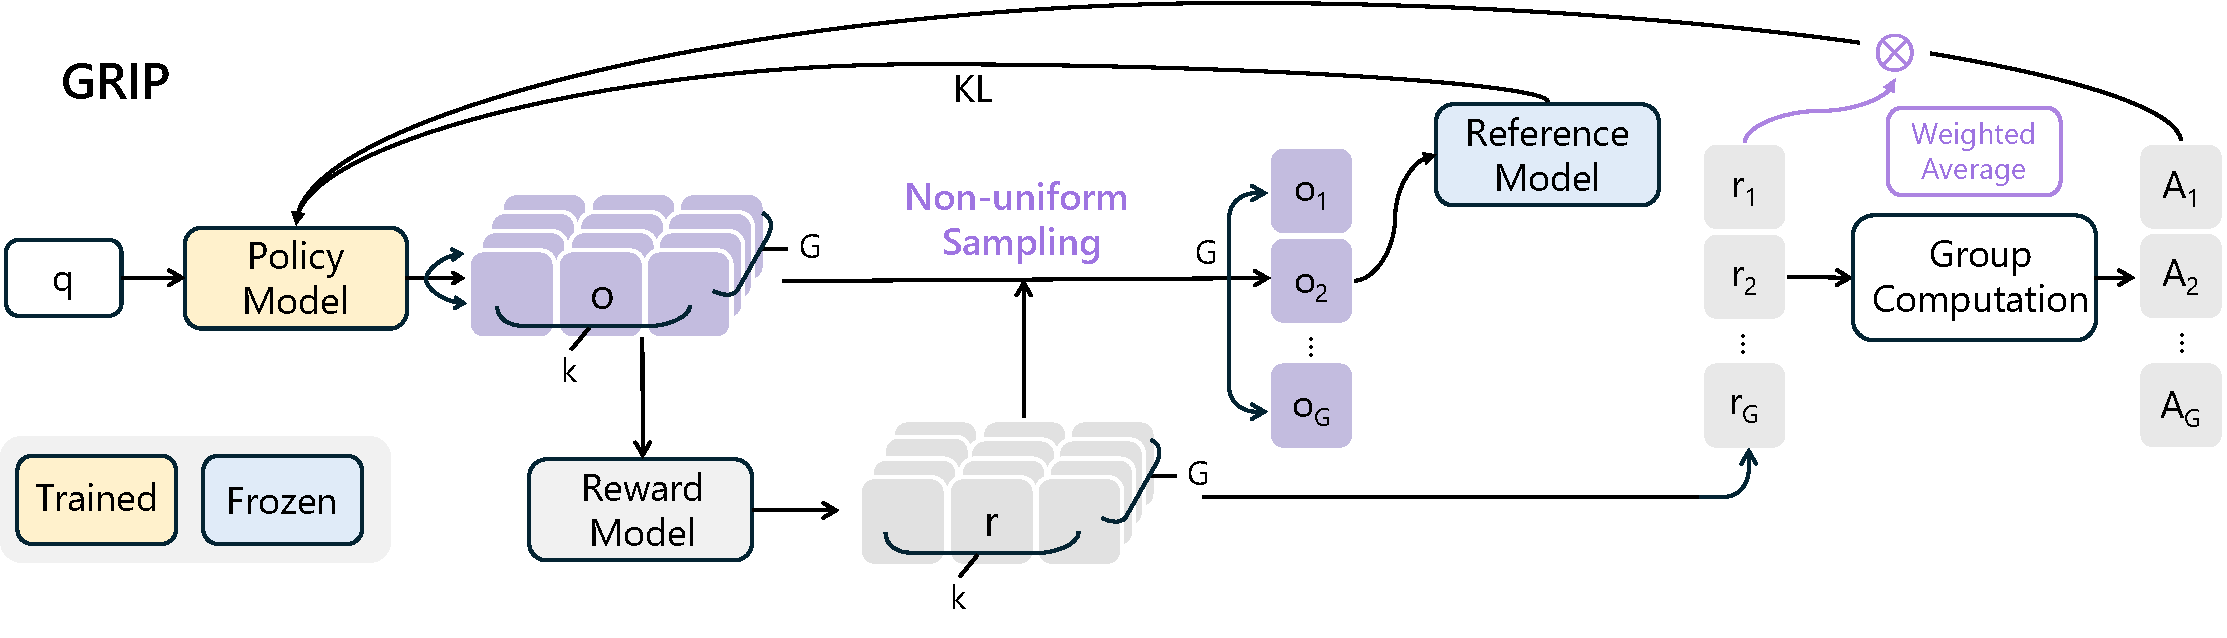
\includegraphics[width=1\textwidth, keepaspectratio]{images/2_grip_.pdf} % 调整宽度    

    \caption{Overview of Group-based Relative Importance for Policy Optimization (GRIP). } % 添加标题
    \label{fig:2_grip} % 添加标签用于引用

\end{figure*}

% \subsubsection{GRIP Optimization Objective}
% The GRIP optimization objective is designed to address the limitations of traditional reinforcement learning methods by integrating a two-stage hybrid sampling mechanism and adaptive weighting within a policy gradient framework. The objective function, formalized in Equation \ref{eq:2}, balances exploration and exploitation while mitigating gradient dilution through structured sampling and trajectory-specific weighting.  

% \paragraph{Two-stage hybrid sampling mechanism.}
% To overcome the exploration-exploitation imbalance inherent in methods like GRPO, GRIP introduces a two-stage sampling strategy. In the first stage, $k \cdot G$ candidate trajectories $\{o_j\}_{j=1}^{k \cdot G}$ are generated from the current policy $\pi_{\theta_{\text{old}}}$, where $k$ controls the size of the rollout space and $G$ denotes the group size. This expansive generation ensures broad exploration of diverse behaviors. In the second stage, a sampling process $\text{Sample}\left(\{o_j\}_{j=1}^{k \cdot G}; R(o_j)\right)$ selects $G$ high-quality trajectories based on their reward $R(o_j)$, prioritizing exploitation of promising regions. These $G$ elite trajectories are then replicated to form the final update set $\{o_i\}_{i=1}^G$, maintaining the original GRPO update scale while amplifying the influence of high-reward samples. This design is mathematically equivalent to an importance-sampled correction of the policy gradient, enabling more stable and efficient updates.  By expanding the search space and focusing on high-quality samples, GRIP achieves a balanced trade-off between exploration and computational efficiency.  More details about the sampling strategy will be discussed in the following sections.

% \paragraph{Adaptive weighting for gradient enhancement.}  
% Traditional uniform weighting like GRPO ($1/G$) across trajectories fails to account for inter-trajectory quality disparities, leading to misleading gradients from low-quality samples and diminished signals for high-quality ones. GRIP addresses this by assigning trajectory-specific weights via a softmax function:  
% \begin{equation}
% w_i^U = \frac{\exp(\hat{x}_{q, o_i})}{\sum_{j=1}^{G} \exp(\hat{x}_{q, o_j})},
% \end{equation}
% where the completion score $\hat{x}_{q, o_i}$ can be flexibly configured. For example, when $\hat{x}_{q, o_i} = R(o_i)$, the weighting amplifies the influence of high-reward trajectories; alternatively, $\hat{x}_{q, o_i}$ can encode uncertainty estimates (e.g., Monte Carlo dropout variance), enabling the model to focus on ambiguous or uncertain samples. This adaptive weighting suppresses noise from low-quality outputs and strengthens gradients from critical trajectories.  

% \paragraph{Formalization of the GRIP objective.} 
% The GRIP objective combines the two-stage sampling and adaptive weighting within a policy gradient framework, as formalized in Equation \ref{eq:2}:  
% \begin{align}
% \mathcal{J}_{\text{GRIP}}(\theta) = 
% &\mathbb{E}_{\substack{q \sim P(Q), \\ \{o_j\}_{j=1}^{k \cdot G} \sim \pi_{\theta_{\text{old}}}(o|q), \\ \{o_i\}_{i=1}^G \sim \text{Sample}\left(\{o_j\}_{j=1}^{k \cdot G}; R(o_j)\right)}} 
% \Bigg\{ 
% \sum_{i=1}^{G} w_i^U  
% \frac{1}{|o_i|} 
% \bigg\{
% \sum_{t=1}^{|o_i|} 
% \min\bigg[ 
% \frac{\pi_\theta(o_{i,t}|q, o_{i,<t})}{\pi_{\theta_{\text{old}}}(o_{i,t}|q, o_{i,<t})} A_i,\nonumber\\
% &
% \text{clip}\Big( \frac{\pi_\theta(o_{i,t}|q, o_{i,<t})}{\pi_{\theta_{\text{old}}}(o_{i,t}|q, o_{i,<t})}, 1-\epsilon, 1+\epsilon \Big) A_i 
% \bigg]
% - \beta \mathbb{D}_{KL} [\pi_\theta || \pi_{ref}] 
% \bigg\} 
% \Bigg\}
% \label{eq:2}
% \end{align}  

% where

% \begin{equation}
%     \mathbb{D}_{KL} \left[\pi_\theta || \pi_{ref}\right] = \frac{\pi_{ref}(o_{i,t}|q, o_{i,<t})}{\pi_\theta(o_{i,t}|q, o_{i,<t})} - \log \frac{\pi_{ref}(o_{i,t}|q, o_{i,<t})}{\pi_\theta(o_{i,t}|q, o_{i,<t})} - 1.
% \end{equation}

% Here, $\epsilon$ and $\beta$ are hyperparameters. $\pi_{\text{ref}}$ is the reference model, typically initialized as the pre-trained model before reinforcement learning begins. The term $o^*$ is selected through a sampling process $\text{Sample}\left(\{o_j\}_{j=1}^{k \cdot G}; R(o_j)\right)$, where $\{o_j\}_{j=1}^{k \cdot G}$ denotes the set of candidate trajectories generated from the current policy $\pi_{\theta_{\text{old}}}$. The hyperparameter $k$ controls the size of the rollout space , while $G$ referred to as the group size. And $A_i$ is the advantage computed using a group of rewards $\{r_1, r_2, \dots, r_G\}$ corresponding to the completion trajectories within each group:

% \begin{equation}
%     A_i = \frac{r_i - \text{mean}(\{r_1, r_2, \dots, r_G\})}{\text{std}(\{r_1, r_2, \dots, r_G\})}.
% \end{equation}



% \subsubsection{Non-uniform Sampling Strategy within the Group}
% To address exploration-exploitation imbalance in methods like GRPO, GRIP introduces a two-stage sampling strategy. First, $k \cdot G$ trajectories $\{o_j\}$ are sampled from the current policy $\pi_{\theta_{\text{old}}}$ to enable broad exploration. Then, the top $G$ trajectories are selected based on reward $R(o_j)$ to emphasize exploitation. These elite trajectories form the final update batch, amplifying high-quality signals while maintaining computational efficiency.
% To further generalize this framework, GRIP supports two distinct sampling strategies:  

% 1. \textbf{Local Random Sampling}: For each input question $q$, we first generate $k$ candidate trajectories $\{o_j\}_{j=1}^k$ by independently sampling from the current policy $\pi_{\theta_{\text{old}}}$. The trajectory with the highest reward $o^* = \arg\max_{1 \leq j \leq k} R(o_j)$ is selected as the elite sample. This process is repeated $G$ times to construct the final set $\{o_i\}_{i=1}^G$. This strategy emphasizes deterministic exploitation of the top-performing sample at each iteration while maintaining computational efficiency.  

% 2. \textbf{Cluster-based Random Sampling}: For each $q$, we generate $k \cdot G$ candidate trajectories $\{o_j\}_{j=1}^{k \cdot G}$. These trajectories are clustered based on their rewards (e.g., reward-binning or K-means clustering), and $G$ trajectories are randomly sampled across clusters to ensure diversity in the final update set. This method balances exploration and exploitation by preserving low-reward but potentially informative samples while still prioritizing high-reward paths.  




